\section{Durchführung}
  \label{sec:Durchführung}
  Der Versuchsaufbau (dargestellt in Abb. \ref{fig:aufbau}) besteht aus einer radioaktiven Quelle die durch zwei Schlitze senkrecht auf die zu untersuchende Folie strahlt, hinter der ein Surface-Barrier-Detektor verbaut ist.
  Der gesamte Aufbau kann mit einer Vakuumpumpe evakuiert werden, und durch ein Feindosierventil auf einen beliebigen Innendruck (bis zum Wiedererreichen des Atmosph"arendrucks) gebracht werden.
  Die Folien k"onnen ausgetauscht werden und auf der Halterung im Aufbau um einen beliebigen Winkel zum einfallenden Teilchenstrahl gedreht werden.
  Als radioaktive Quelle wird das Isotop $^{241}\text{Am}$ mit Halbwertszeit $\tau=432,2$ Jahre verwendet, welches ausschlie"slich unter $\alpha$-Zerfall in $^{237}\text{Np}$ zerf"allt, mit einer mittleren kinetischen Energie der $\alpha$-Teilchen/Heliumkerne von $E_{\alpha}=\SI{5,486}{\mega \electronvolt}$.
  Als Folien stehen zu verf"ugung: zwei Goldfolien mit Dicke $d=\SI{2}{\micro \meter}$ und $\SI{3}{\micro \meter}$, eine Aluminiumfolie mit $d=\SI{1}{\micro \meter}$ und eine $\SI{3}{\micro \meter}$ dicke Bismuthfolie.

  Zum Messen des Energieverlusts der $\alpha$-Teilchen, k"onnen am Oszilloskop Spannungsausschl"age der registrierten  $\alpha$-Teilchen angezeigt werden. Die H"ohe der Ausschl"age ist dabei proportional zur Energie $E_{\alpha,nach}$ der Teilchen nach dem Durchlaufen der verbauten Folie.
  Die Pulse k"onnen am Oszilloskop auch gemittelt werden.

  Zur Messung der Z"ahlrate $I(\theta)$ als Funktion des Streuwinkels $\theta$ steht ein Z"ahler mit verbundenem Timer zu Verf"ugung.

  Vor Beginn der eigentlichen Messung wird die Aktivit"at der Am-Probe gemessen, indem $\SI{200}{\second}$ lang die regestrierten Teilchen beim Detektor (ohne Folie) gemessen werden.

  \begin{figure}
    \centering
    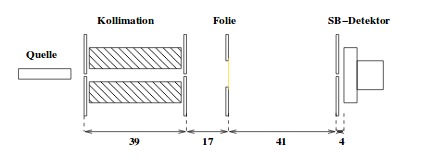
\includegraphics[height=4cm]{bilder/aufbau.png}
    \caption{Der Versuchsaufbau mit Abmessungen \cite{Anleitung}}
    \label{fig:aufbau}
  \end{figure}



  \subsection{\texorpdfstring{Bestimmung der Foliendicke einer Goldfolie durch Energieverlustmessung der $\alpha$-Teilchen}{Bestimmung der Foliendicke einer Goldfolie durch Energieverlustmessung der alpha-Teilchen}}
    Um in der Auswertung die Dicke $d$ der verwendeten Goldfolie ($d_{theo}=\SI{2}{\micro \meter}$) mit der Bethe-Bloch-Gleichung zu bestimmen, wird die Pulsh"ohe der Detektorpulse also Funktion des Kammerdruckes (also als Funktion von $N$) gemessen, einmal mit und einmal ohne Folie.

    Am Oszilloskop wird der Trigger auf $\SI{600}{\milli \volt}$ eingestellt, sodass das Rauschen nicht als Signal detektiert wird.
    Die H"ohe der Ausschl"age wird nicht mit der Mittelwertsfunktion sondern manuell mit dem Cursor abgelesen.

    Nun wird mit und ohne Folie je die Spannungsh"ohe der Ausschl"age und der zugeh"orige Kammerdruck notiert.
    Dabei wird vom Vakuum ausgegangen und so lange Messwerte genommen, bis keine Auschl"age mehr zu sehen sind, das hei"st die Energien der $\alpha$-Teilchen durch den h"oheren Luftdruck zu gering sind, um vom Trigger regestriert zu werden.
    Insgesamt werden dadurch je 5 Wertepaare (Pulsh"ohe,Kammerdruck) vom Vakuum bis $\SI{140}{\milli \bar}$ aufgenommen.




  \subsection{Vermessung des Rutherford-Streugesetzes}
    Um den experimentellen Verlauf der Rutherford-Streuformel zu bestimmen zu k"onnen wird nun die Z"ahlrate $Z(\theta)$ der Heliumkerne nach der Folie als Funktion des Streuwinkels $\theta$ gemessen (f"ur die $\SI{2}{\micro \meter}$-Goldfolie).
    Dazu wird das Oszilloskop vom SB-Detektor abgest"opselt und statdessen der Z"ahler angeschlossen und die Kammer ist durchgehend evakuiert.
    Bei jedem ($\theta$, $Z(\theta)$)-Messwertepaar wird bis ungef"ahr 1000 Counts/regestrierte Teilchen gemessen, um den Fehler zu minimieren.

    Es wird im Bereich von $\SI{0}{\degree}$ bis $\SI{3}{\degree}$ in $\SI{0,2}{\degree}$ Schritten die Z"ahlrate und zugeh"origer Winkel notiert, danach nur noch f"ur die Winkel $\SI{7}{\degree},\SI{10}{\degree},\SI{15}{\degree},\SI{20}{\degree}$.


  \subsection{Nachweis von Mehrfachstreuungen und und $Z$-Abh"angigkeit der Rutherford-Streuformel}
    Es werden f"ur die restlichen drei Folien ($\SI{1}{\micro \meter}$ Aluminium, $\SI{3}{\micro \meter}$ Bismuth und $\SI{3}{\micro \meter}$ Gold) die Z"ahlrate $Z(\theta)$ in Abh"angigkeit des Winkels $\theta$ gemessen und notiert, f"ur die Winkel $\SI{0}{\degree},\SI{3}{\degree},\SI{7}{\degree}$.
    Die Messungen werden wie vorher im Vakuum durchgef"uhrt.
